\section{Problem Model}

\begin{frame}{Problem abstraction}{The optimization model}

\begin{figure}
\centering
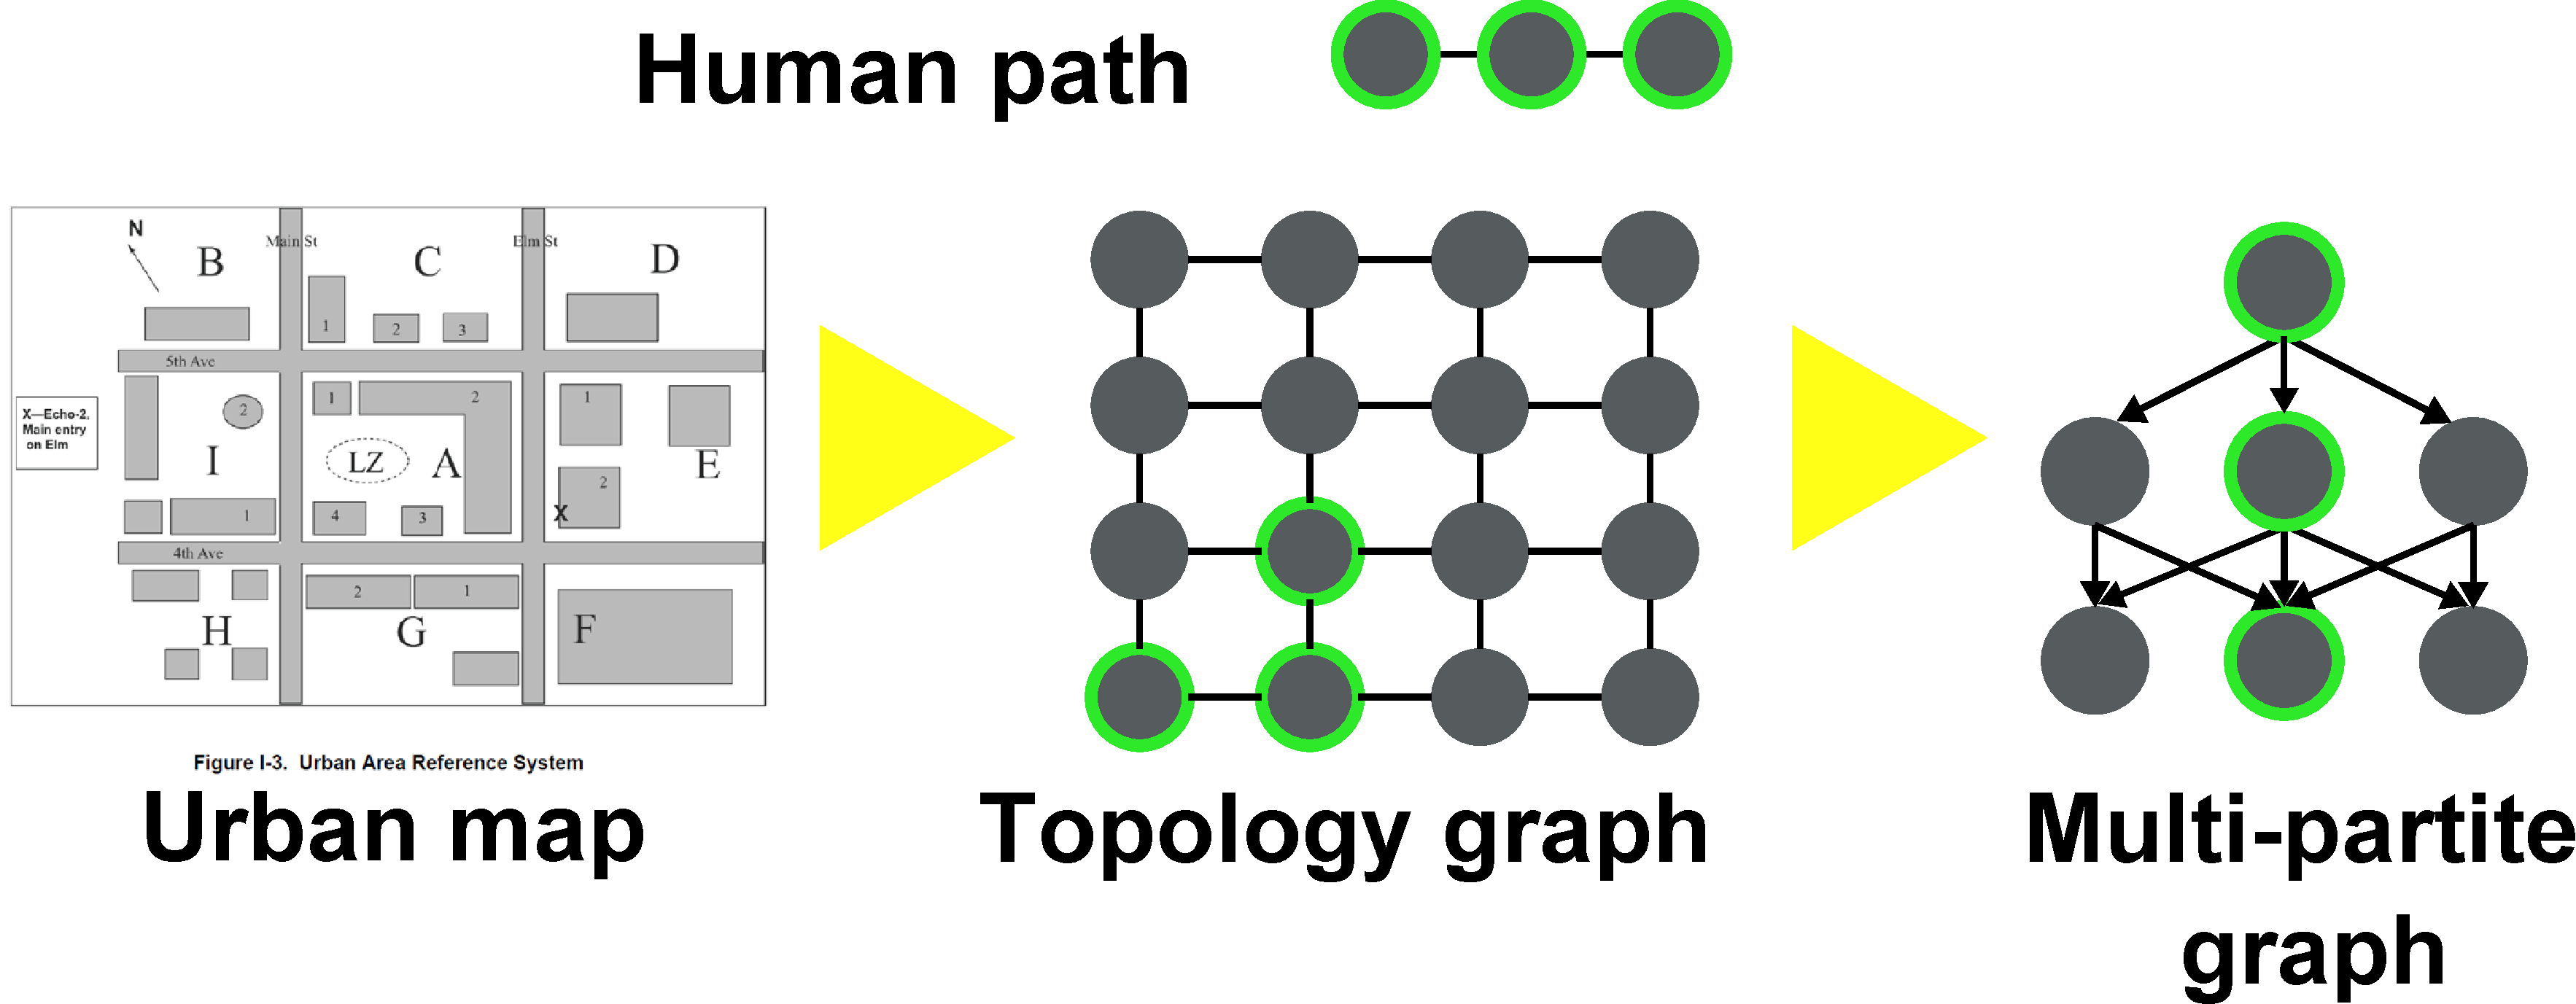
\includegraphics[width = 0.9\textwidth]{./figure/layers}
%\caption{A layered problem processing.}
\end{figure}

\end{frame}

\begin{frame}{The multi-partite graph}{The optimization model}

\begin{columns}

\column{.6\textwidth}
\begin{minipage}[c]{\textwidth}
\begin{figure}
\centering
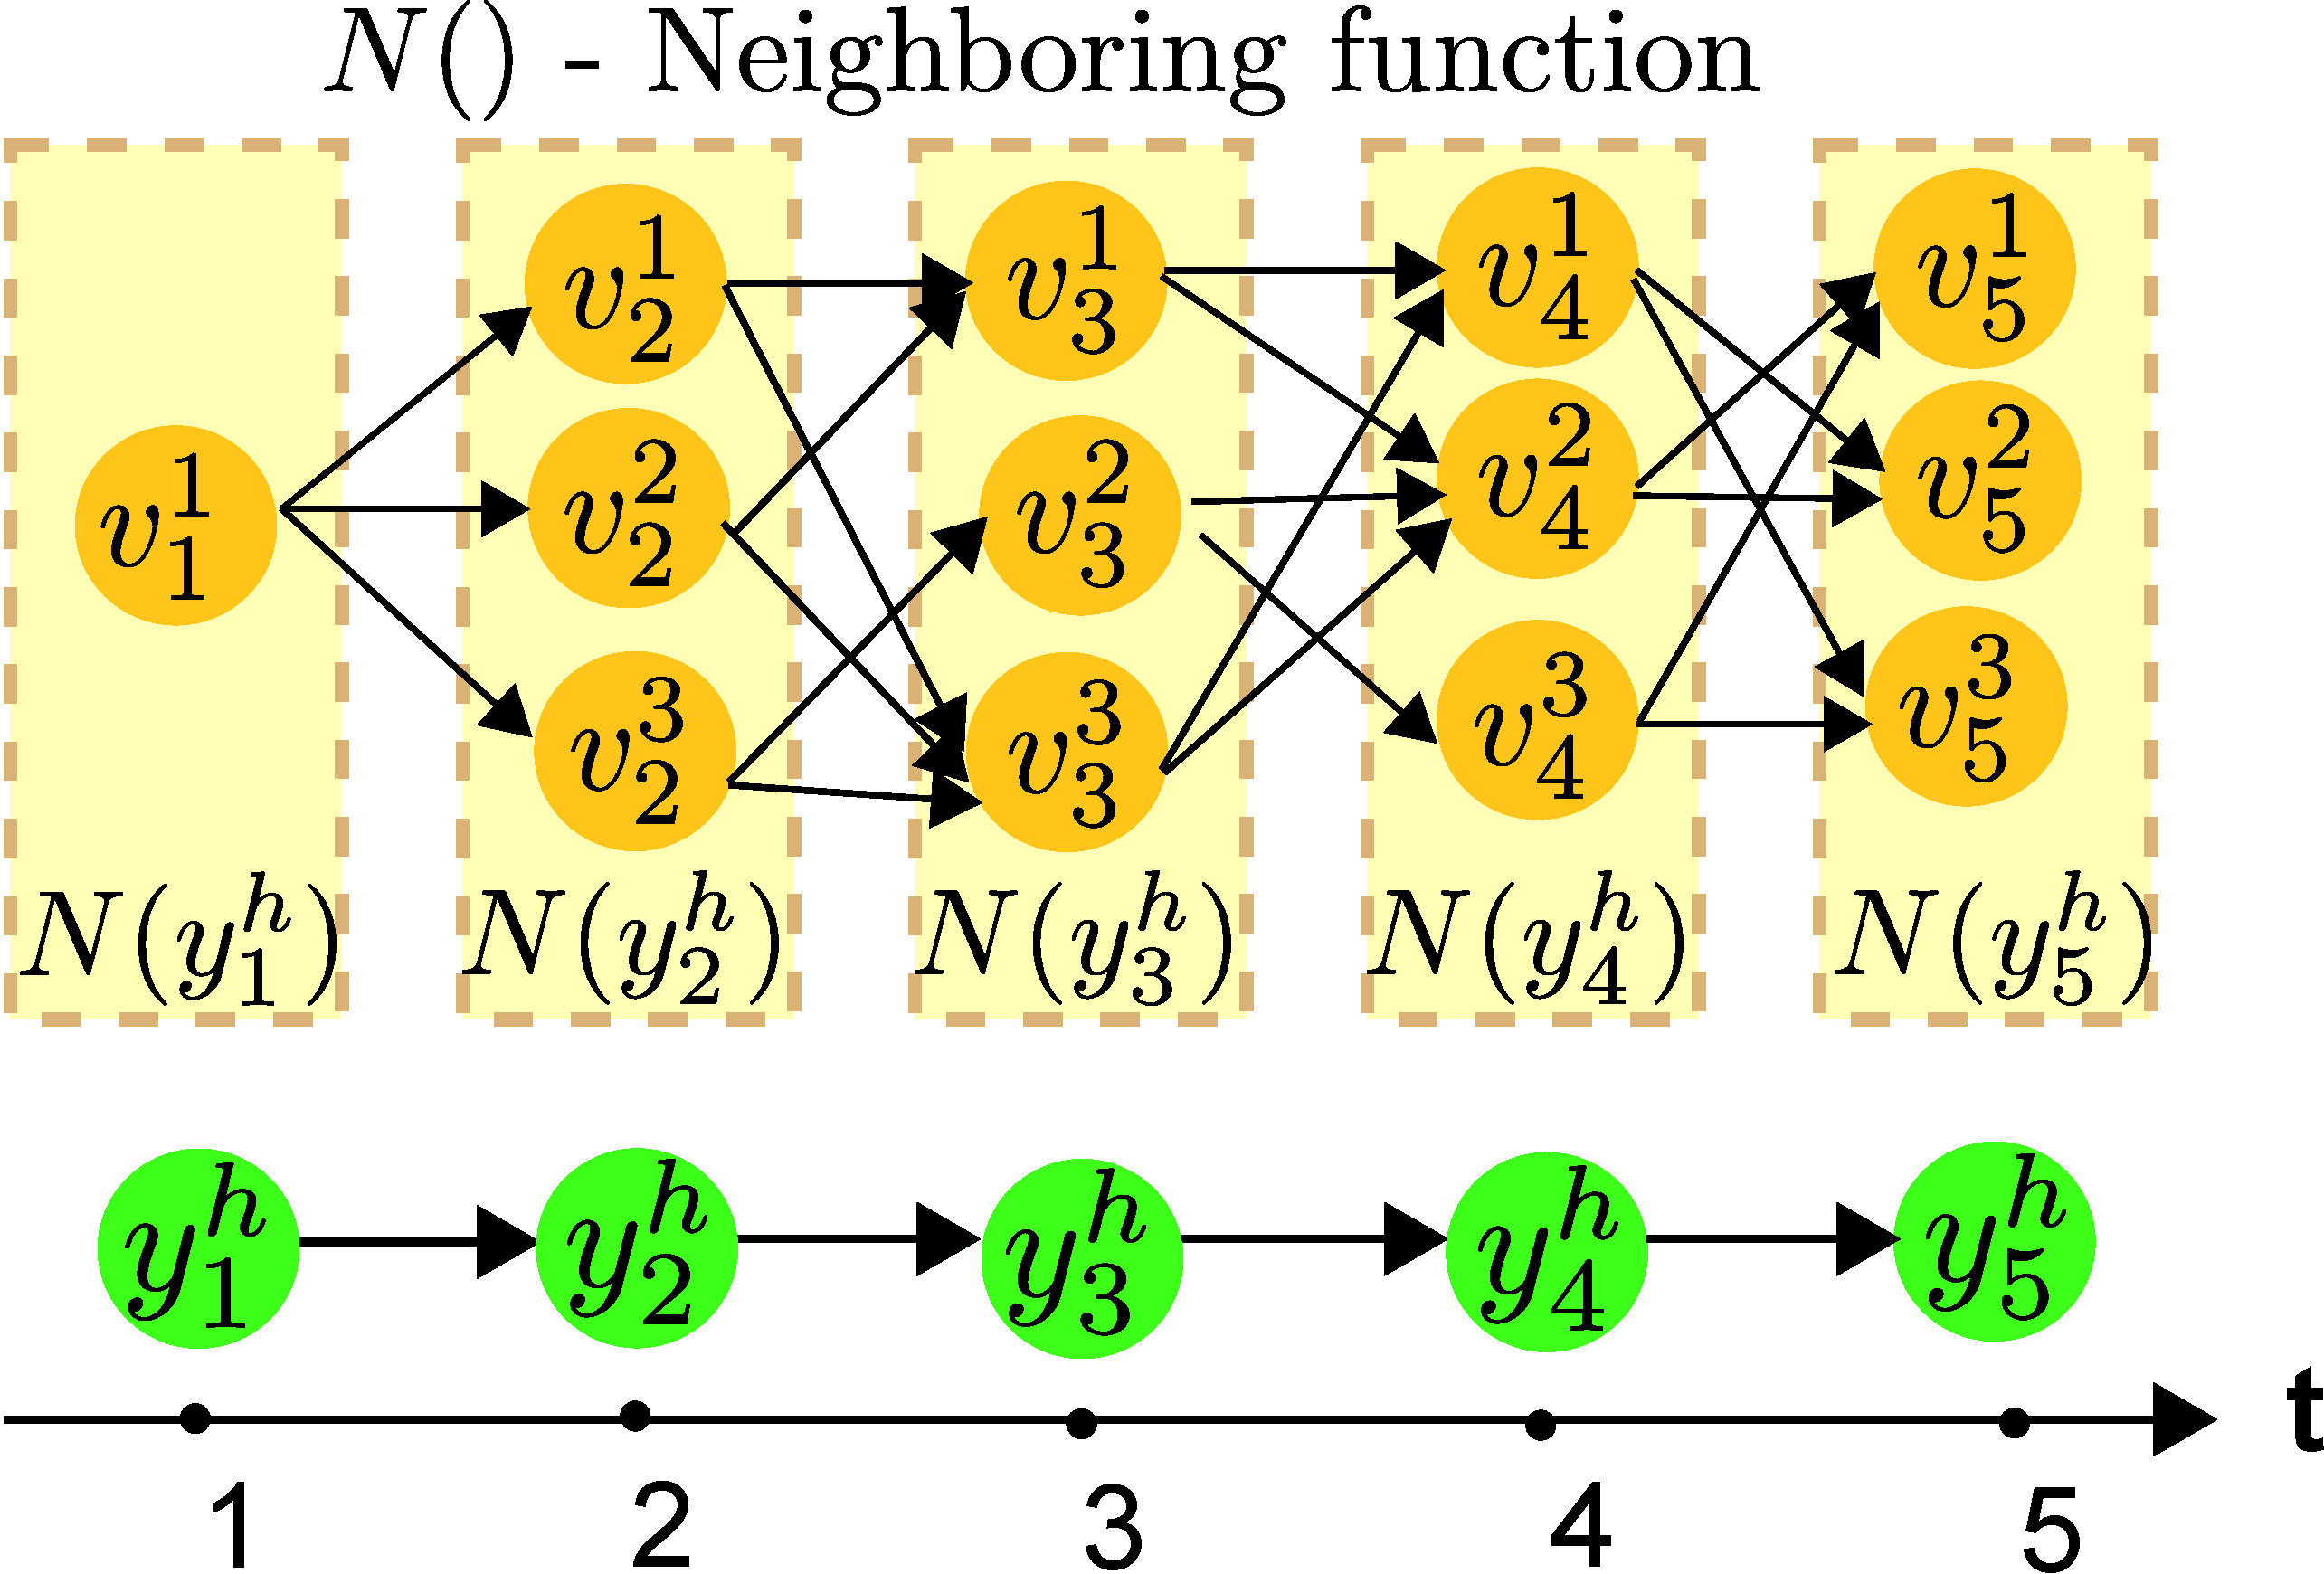
\includegraphics[width = \textwidth]{./figure/MultiPartite}
%\caption{A multi-partite graph generated from human constraint.}
\end{figure}
\end{minipage}

\column{.4\textwidth}
\begin{minipage}[c]{\textwidth}
\begin{itemize}
\item time-space synchronization
\item connection determined by discretized map
\end{itemize}
\end{minipage}

\end{columns}

\end{frame}

\begin{frame}{A pruning process}{The optimization model}

\begin{columns}
\column{.45\textwidth}
%\begin{minipage}
%\begin{block}
Reachable
%\end{block}
%\end{minipage}

\column{.45\textwidth}
%\begin{minipage}
%\begin{block}
Non-terminating
%\end{block}
%\end{minipage} 

\end{columns}

\begin{columns}

\column{.45\textwidth}

\begin{block}{Forward pruning}
$ \forall t \in \{ 2, \cdots T \}, $ \\
$ \forall v \in V(t), deg^{-}(v) > 0 $

\begin{figure}
\centering
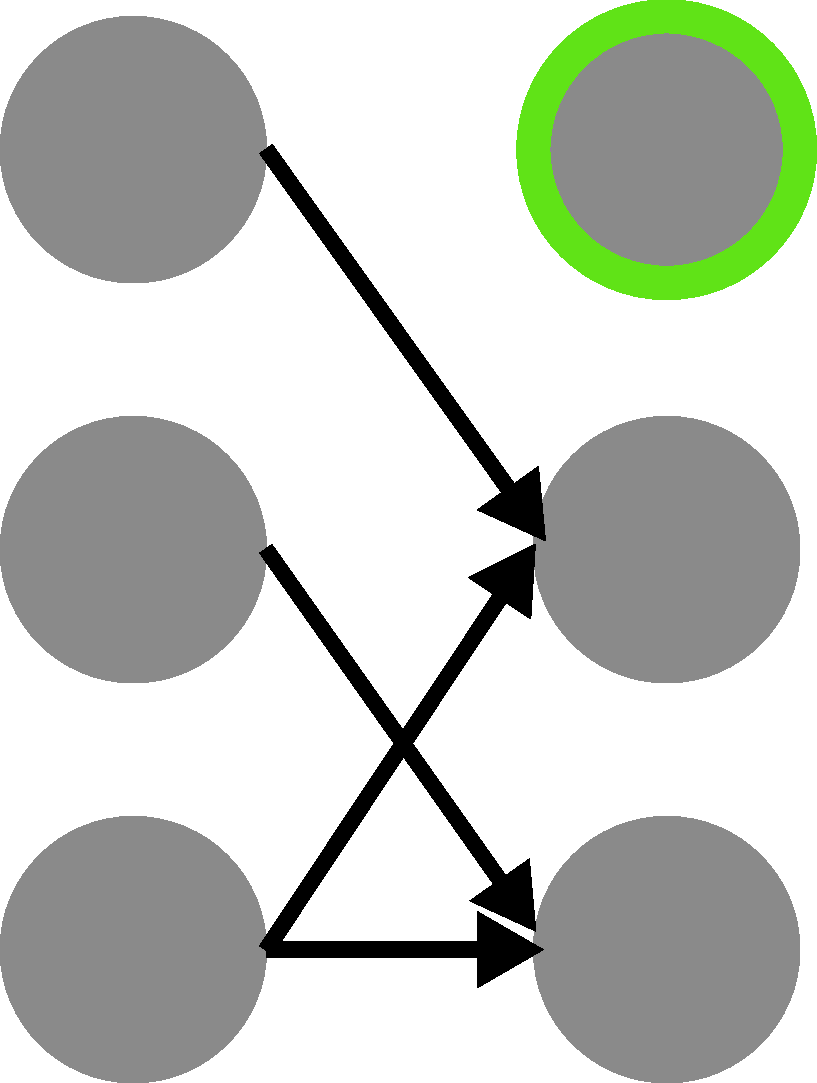
\includegraphics[width = 0.4\textwidth]{./figure/forward_prune}
\end{figure}

\end{block}

\column{.45\textwidth}

\begin{block}{Backward pruning}

$ \forall t \in \{ 1, \cdots T-1 \}, $ \\
$ \forall v \in V(t), deg^{+}(v) > 0 $

\begin{figure}
\centering
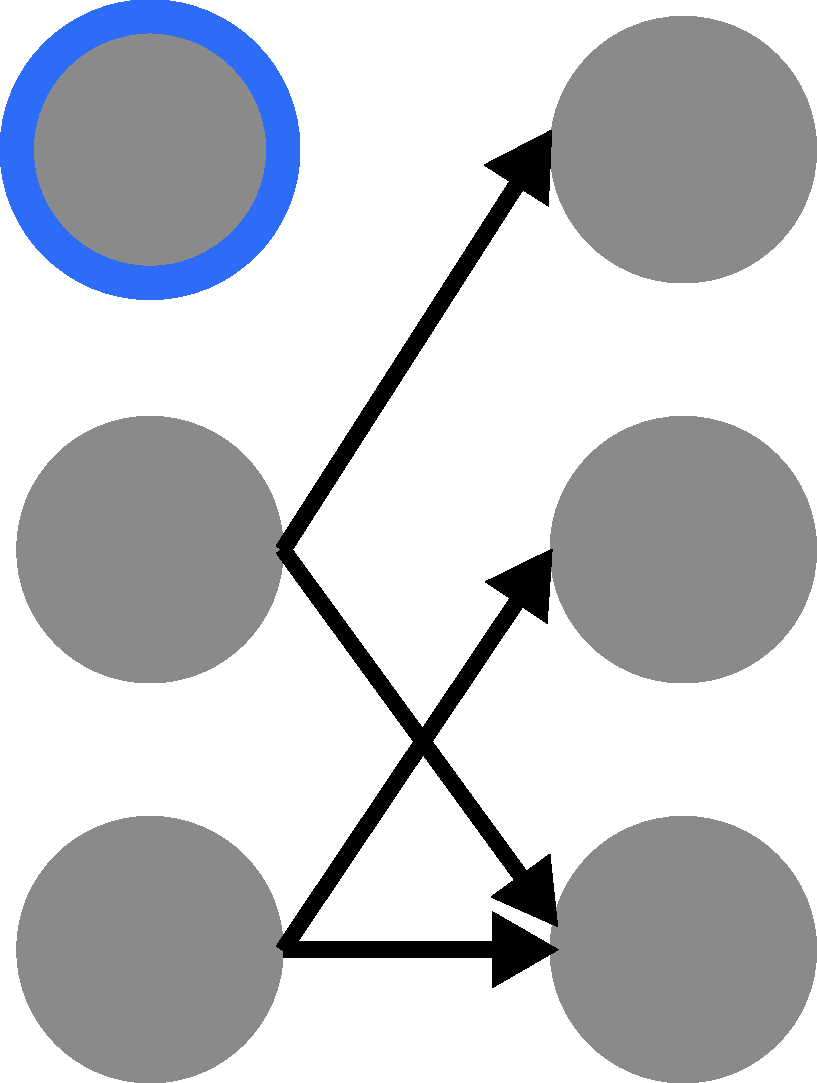
\includegraphics[width = 0.4\textwidth]{./figure/backward_prune}
\end{figure}

\end{block}

\end{columns}

\end{frame}

\begin{frame}{Obstacles}{The optimization model}

\begin{figure}
\centering
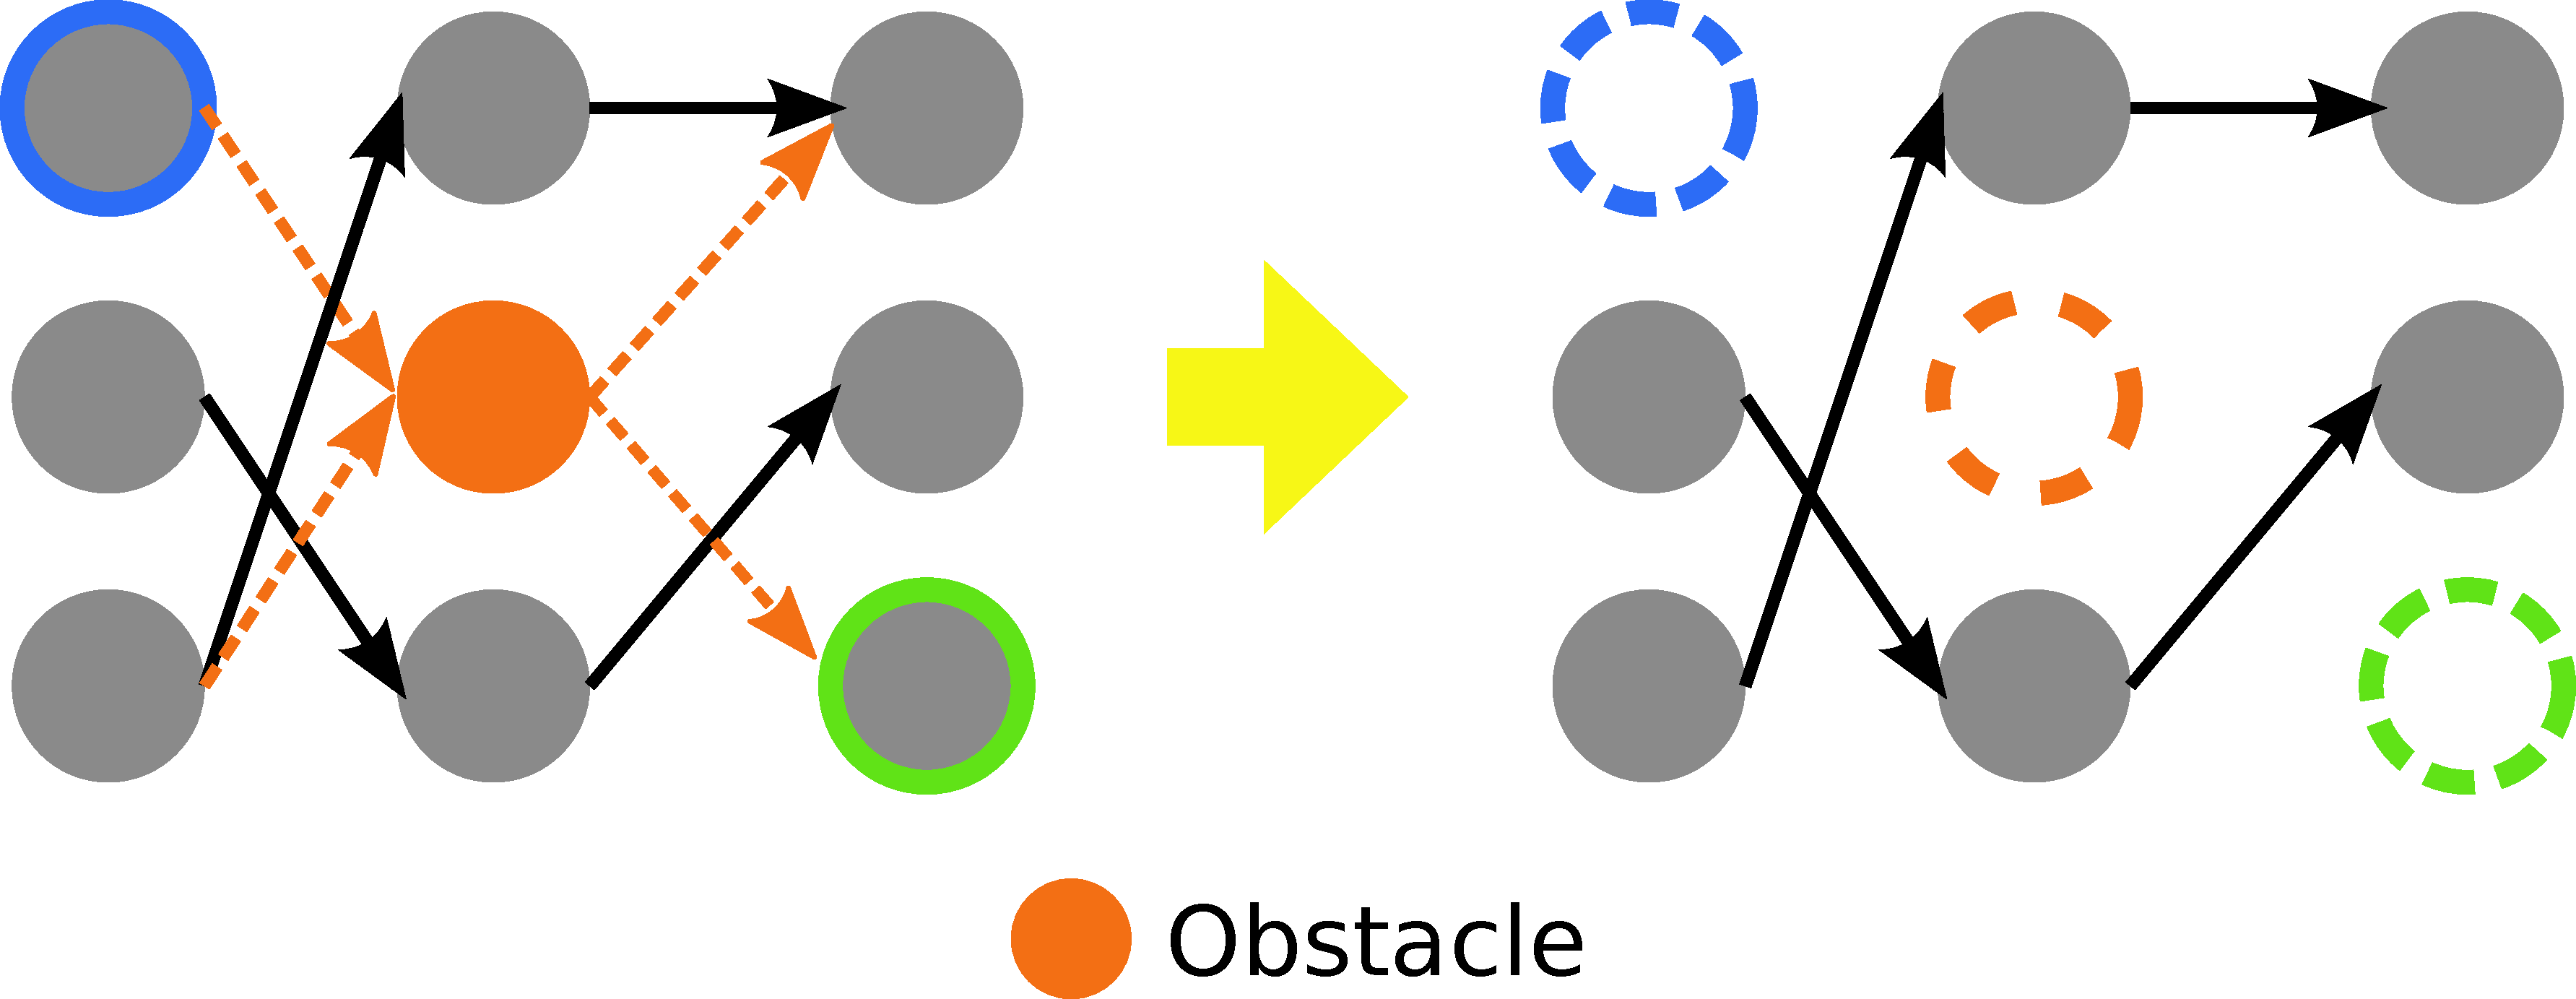
\includegraphics[width = 0.8\textwidth]{./figure/obstacle}
\end{figure}

\end{frame}

\begin{frame}{Submodular orienteering on a multi-partite graph}{The optimization problem}

\begin{equation}
\nonumber
\begin{aligned}
Objective: & X^{*} = \argmax_{X} \: f(X); \\
Constraint: & |X| = T, x_{t} \in V(t), (x_{t}, x_{t+1}) \in E.
\end{aligned}
\end{equation}

\end{frame}